
\documentclass[a4paper 12pt]{article}
\usepackage{enumerate}
\usepackage{amsmath}
\usepackage[utf8]{inputenc}
\usepackage{csquotes}
\usepackage{xcolor}
\usepackage{tikz}
\usepackage{listings}
\usepackage{epigraph}
\usepackage[linguistics]{forest}
\usepackage[boxed,linesnumbered]{algorithm2e}
\usepackage{varwidth}
\usepackage{algpseudocode}
\usepackage{tikz-qtree}
\usepackage[scaled]{beraserif}
\usepackage{graphicx}
\usepackage{hyperref} 
\graphicspath{ {./images/} }
%%\usepackage{bera}
%% Another possibility is
%% \usepackage[scaled]{beraserif}
\usepackage[T1]{fontenc}
%%\usepackage[legalpaper, total={6in, 8in}]{geometry}
\usepackage[utf8]{inputenc}
\title{\vspace{50mm}\textbf{\huge Nearest Vocational Job Finder \\ \huge Software Lab Project}}
\author{\LARGE PhantomTroupe \\ [1ex]
\normalsize 203050036: Ajay Sarup Jain\\
\normalsize 203050078: Mahendra Patel\\
\normalsize 203050009: Ajay Shyamsunder\\
\normalsize 203050099: Polu Varshith\\
\normalsize 203051001: Avijit Darshal} 

\date{\Large 9 September, 2020}

\begin{document}
\maketitle
\thispagestyle{empty}
\clearpage
\pagenumbering{arabic} 
\newpage
\tableofcontents
\newpage
\section{\textbf{Introduction}}
Nearest vocational job finder is a website which is designed for the people who has difficulty in finding vocational job like Electrician, Plumbing etc. There are people who posses relevant skills but don't have the medium to find such jobs. This Platform will help such people to find the jobs in their nearby area related to their skills which will help them to earn money. The existence of such platform are even more required in a situation like covid-19 in which many people have lost their jobs. This web app will also be helpful to job provider as this will also help them to get their work done at reasonable price.\\

This web application which acts as a platform to publish , identify and optimistically match service providers to service receivers based on their location, job start time, job start date, skill required etc. In this app a user can register as a one out of three profile type, He can be job provider, job seeker or can be both. Depending on his profile type his view of the website is slightly changed. Job seeker and both profile type can see job sorted job notification and manage their applied job  whereas job provider and both profile type can post a job and manage job responses. The platform is designed keeping in mind ease of usage so it is kept very simple.\\

\newcommand{\latex}{\LaTeX\xspace}


 \section{\textbf{Motivation}}
In the wake of the global pandemic, there has been a huge disturbance in the service market, both organized and unorganized. The organized sector from some time now has had many platforms (like Monster India, Indeed .etc) to publish and find stable full-time work. But such platforms are not appropriate to post nearby vocational jobs like Plumbing, Electrician, Nursing aides, Carpenters etc. These jobs arise at the need of the hour and current location of the service provider as well as job location is of utmost importance. Our idea is to develop a web application which can act as a middleman for service exchange in these sectors. 


\newpage
\section{\textbf{Dependencies}}
\begin{itemize}
\item Python3
\item Django
\item Postgresql


\end{itemize}


\newpage
\section{\textbf{User Documentation}}
\begin{itemize}
\item sudo apt-get install python3.6\\
To install Django on ubuntu, run the following command in your terminal.
\item pip3 install django\\

\item install postgresql in your system\\
to download the postgresql click on the below link : \\
\href{https://www.postgresql.org/download/}{https://www.postgresql.org/download/}\\
after installation:\\
\begin{enumerate}
    \item create database with name NVJF with default user postgre and password="1234"(without quotes)
    \item check your port no in settings.py
\end{enumerate}
\item pip3 install django
\item pip3 install social-auth-app-django
\item pip3 install psycopg2 \\ 
One needs to git clone the project. After that open terminal in main directory and run following commands.
\item python3 manage.py makemigrations
\item python3 manage.py migrate
\item python3 manage.py runserver
All the functionalities and how to use them is depicted ahead.

\end{itemize}


\subsection{Login Page}
The user will see this page whenever he visited a website. He can login using his G-mail account or create one at that time if he don't one.
\vspace{15mm}
\begin{center}
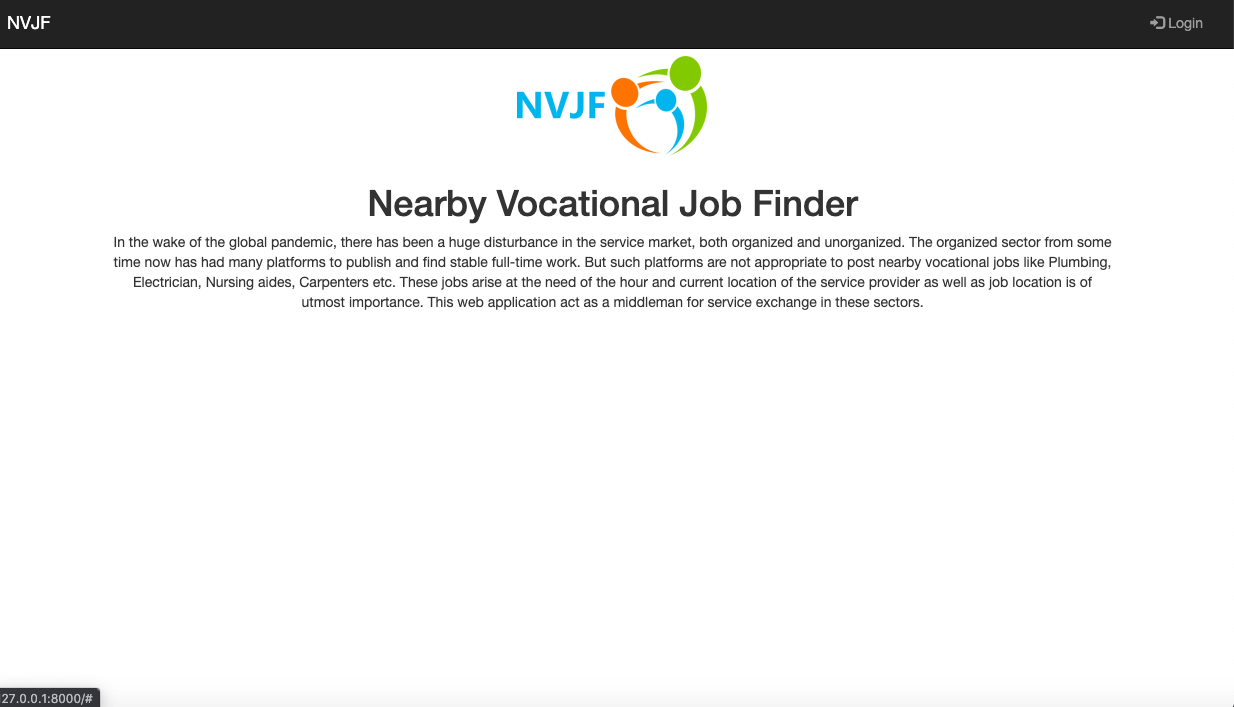
\includegraphics[width=15cm, height=10cm]{sign_in.png}
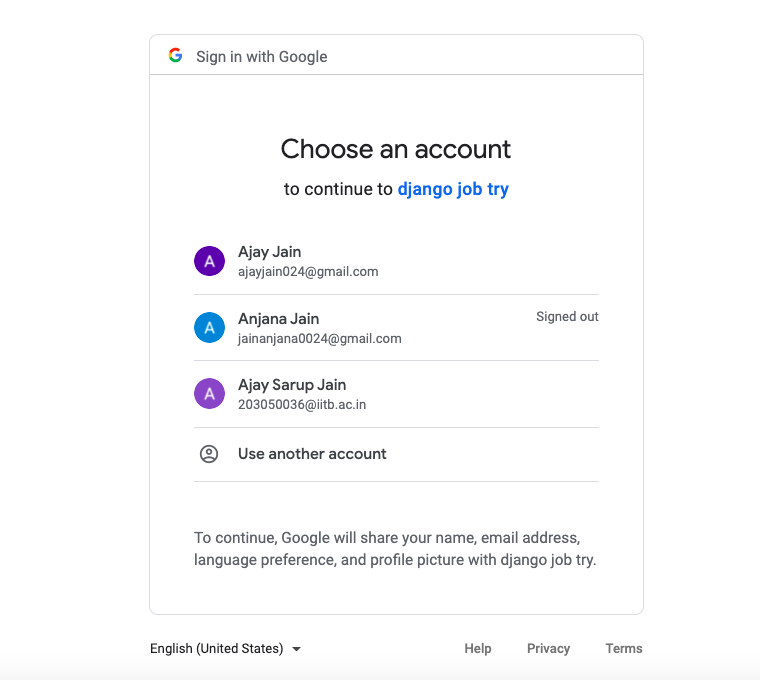
\includegraphics[width=15cm, height=10cm]{google.png}
\end{center}

\newpage
\subsection{Make profile}
The first time user has to fill a small form which will capture some important details and save it in our server.
\begin{center}
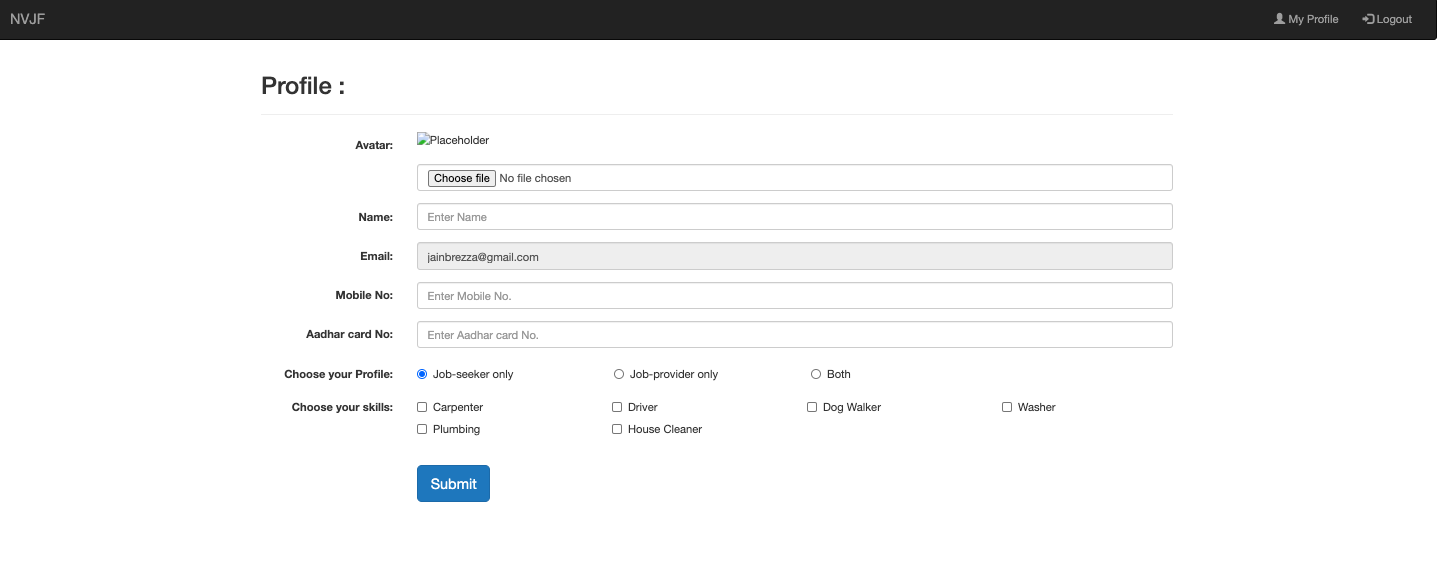
\includegraphics[width=15cm, height=10cm]{makeprofile.png}
\end{center}




\subsection{Job feed notification}
If user is registered as job-seeker or both as a profile type, both will we re-directed to this page.
This was the page where all new posted job was seen in a sorted order of distance . Here user can also apply various filter like price, skills required or by typing relevant words in search box. This will help him to find relevant job easily.\\

This job feed Notification is seen by user whose profile type is both. for a person whose profile type is Job seeker will see same page but less option in navigation bar as he will not be able to post jobs.\\

First image shown below is view seen by profile type both and second image that is below it is view seen by profile type job seeker only. You can notice the only major difference is in navigation bar.\\

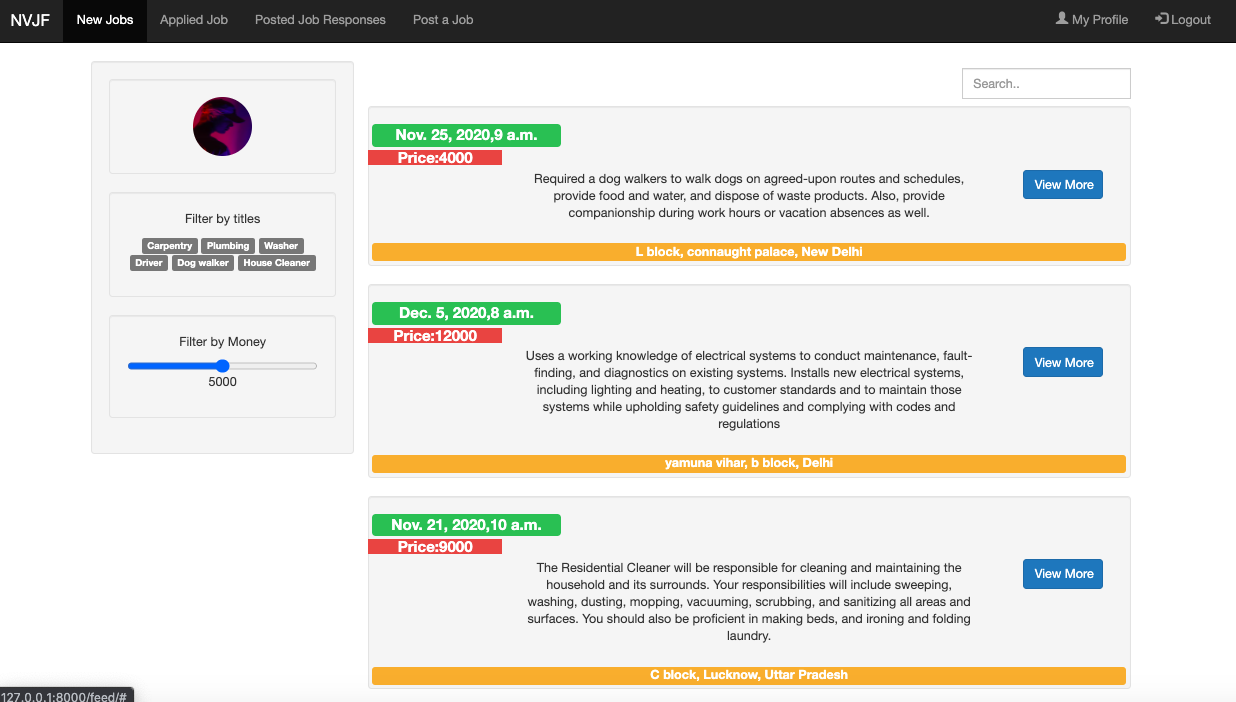
\includegraphics[width=15cm, height=10cm]{feed view for both.png}
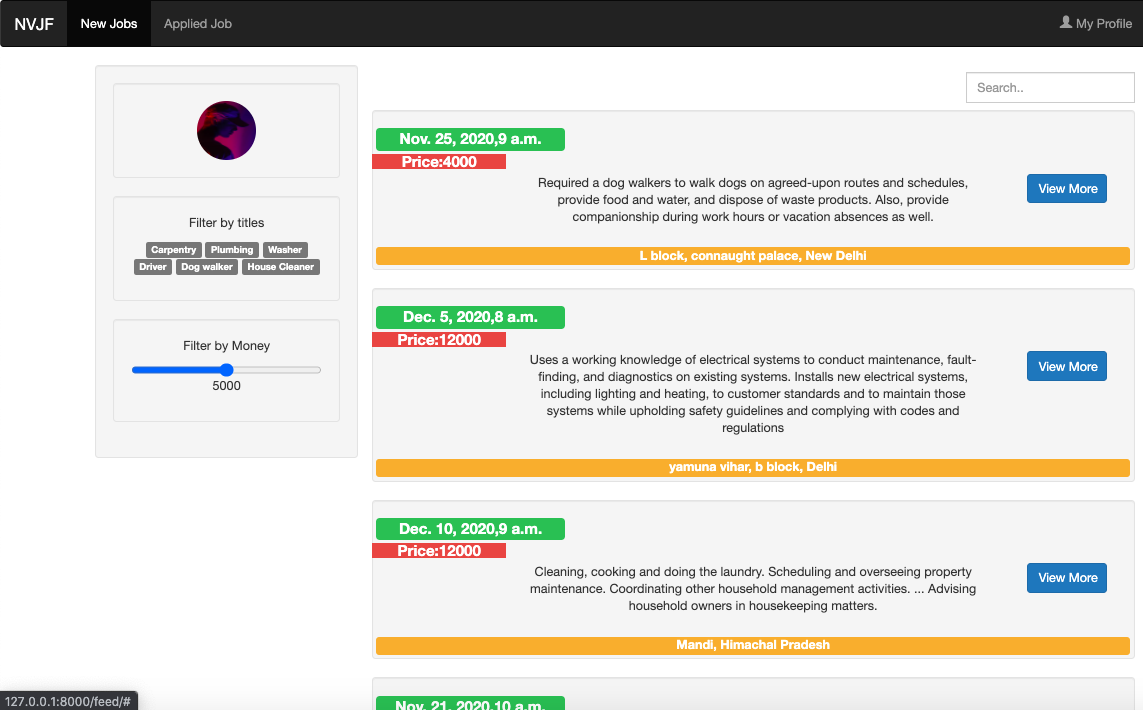
\includegraphics[width=15cm, height=10cm]{feed view for job seeker.png}


\subsection{Job Details}
On any job shown in New job notification page above if you click on view more button then the whole description of that job with images related to the work to be done, address where job is located and details of the job provider can be seen. Through this page job seeker can apply for the job through the portal by clicking on apply button which is at the bottom of the page\\

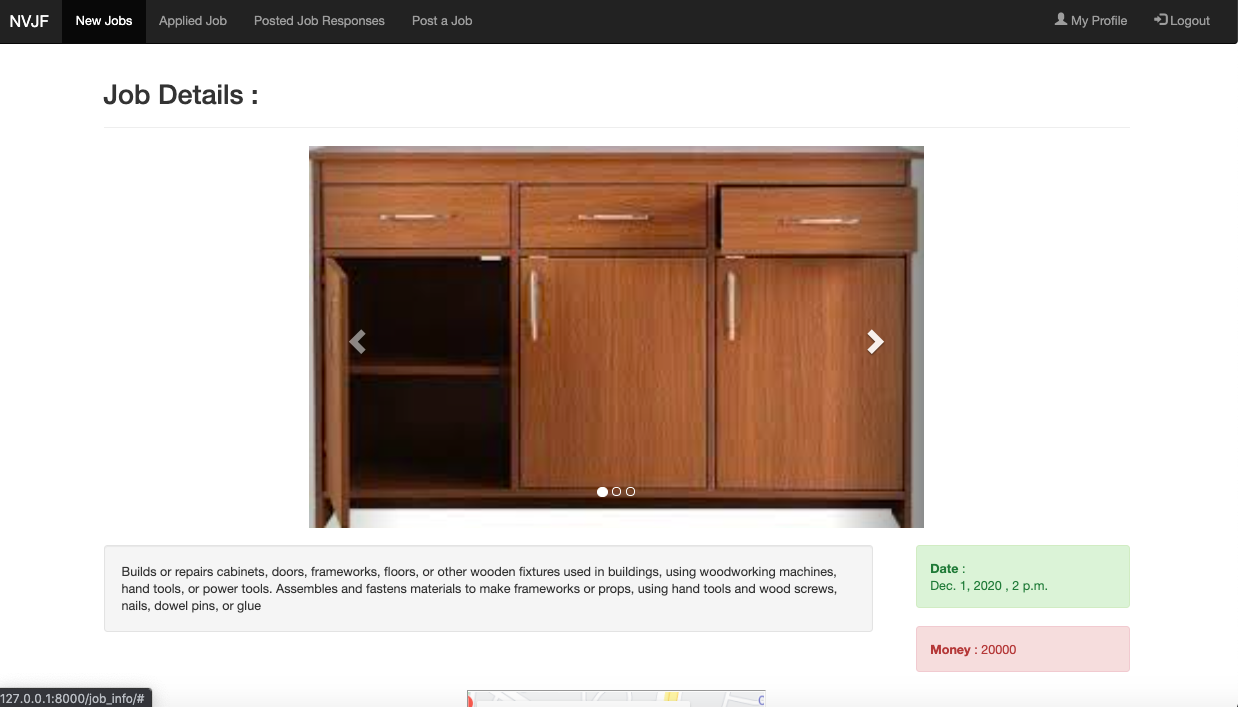
\includegraphics[width=15cm, height=8cm]{Job details 1.png}
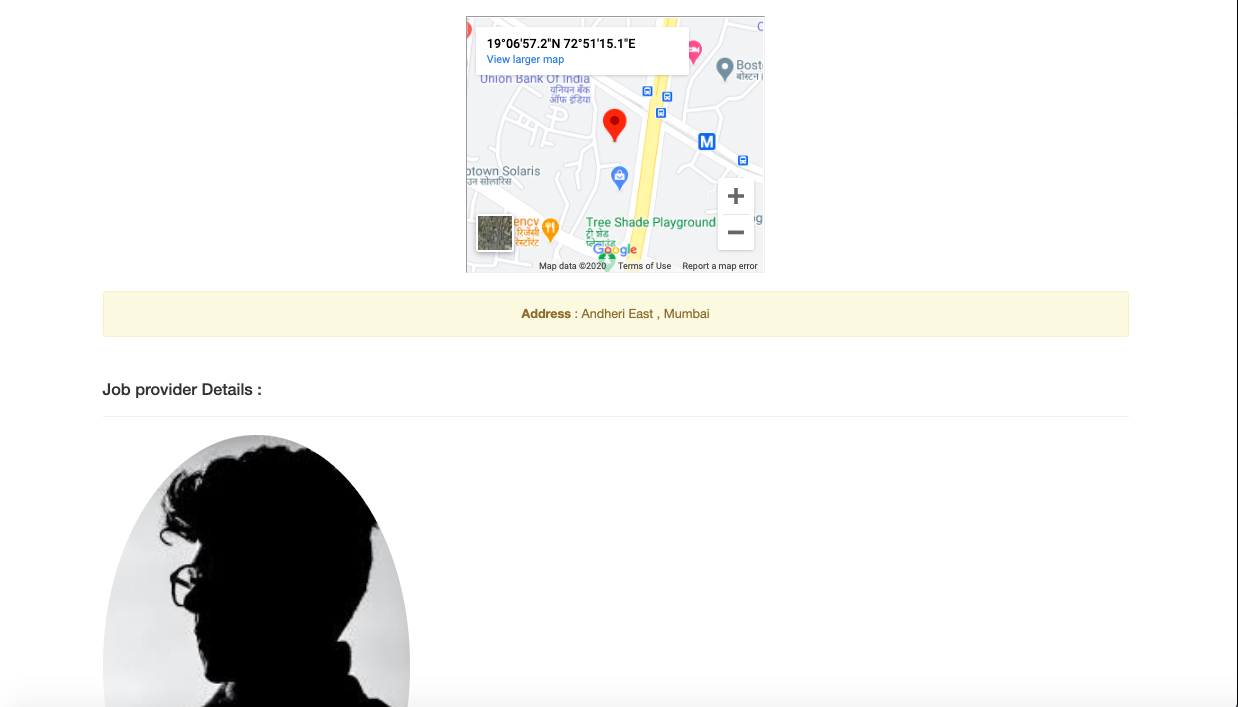
\includegraphics[width=15cm, height=8cm]{job details 2.png}
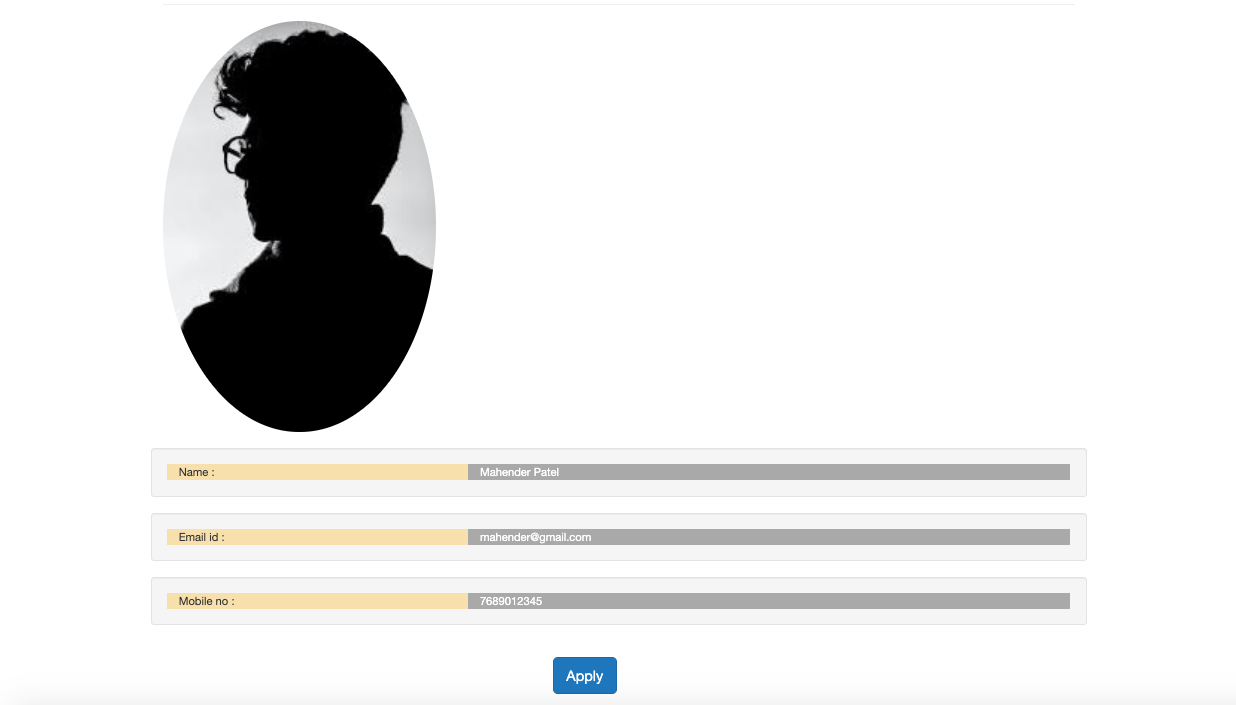
\includegraphics[width=15cm, height=8cm]{job details 3.png}

\subsection{Applied Job}
In the navigation you can see the options of Applied job. Using this option you will be able to track the status of your job whether your job is Approved or its approval is still waiting. Here you can also see the jobs you have successfully completed in past and the jobs you have applied to in past but not able to get. In page he can also able to delete the job he has applied for by clicking on delete button.\\

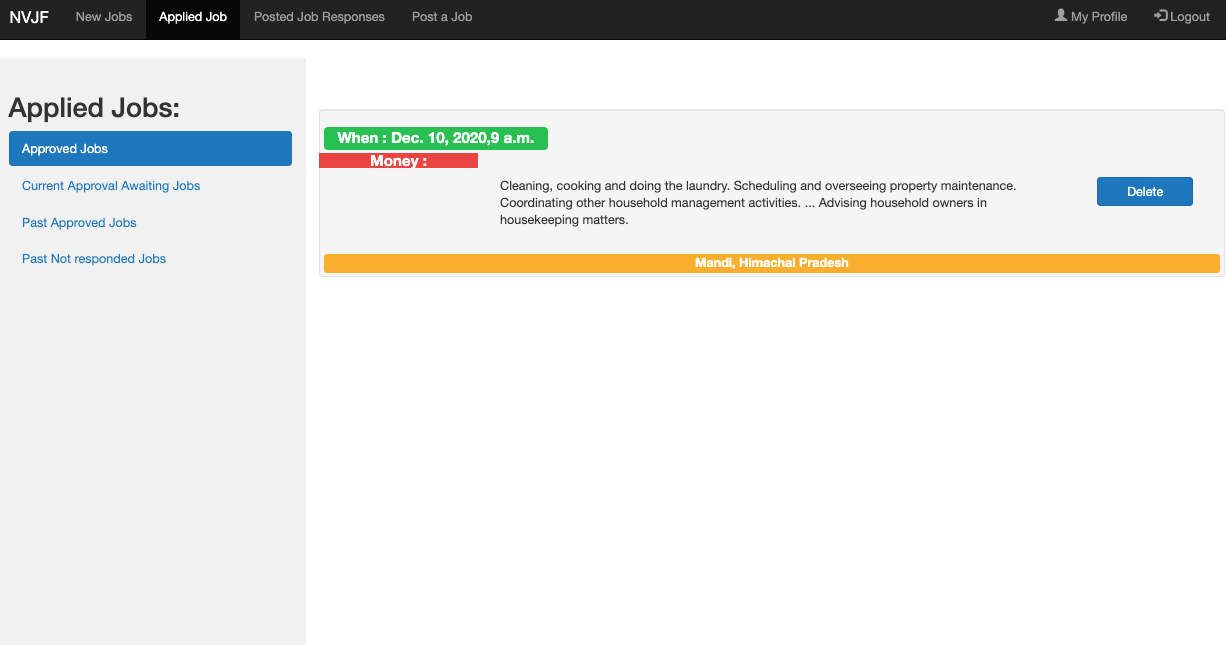
\includegraphics[width=15cm, height=8cm]{applied job approved.png}


\subsection{Post a Job}
This option in navigation is visible only if your profile type is both or job provider. Using this you will be able to post a new job for which you are looking for people. This is a simple form which required to fill small details like job description, address,date,time, price and relevant image related to work. \\

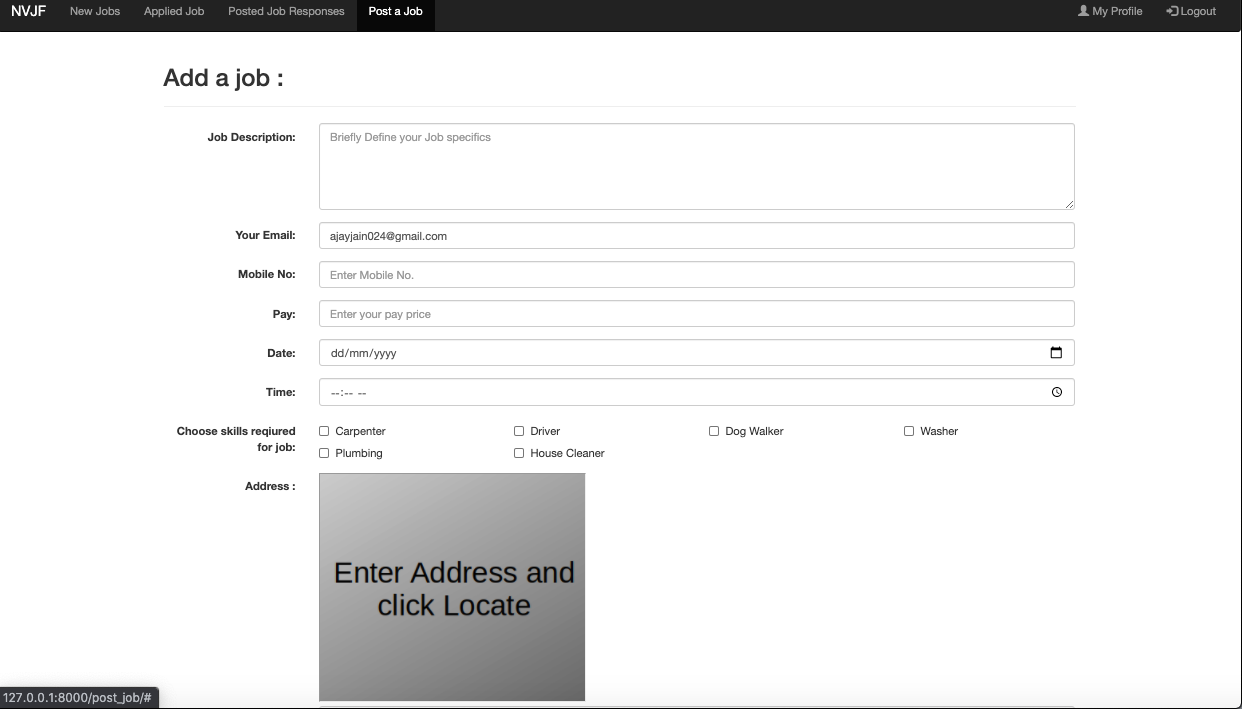
\includegraphics[width=15cm, height=8cm]{post job 2.png}
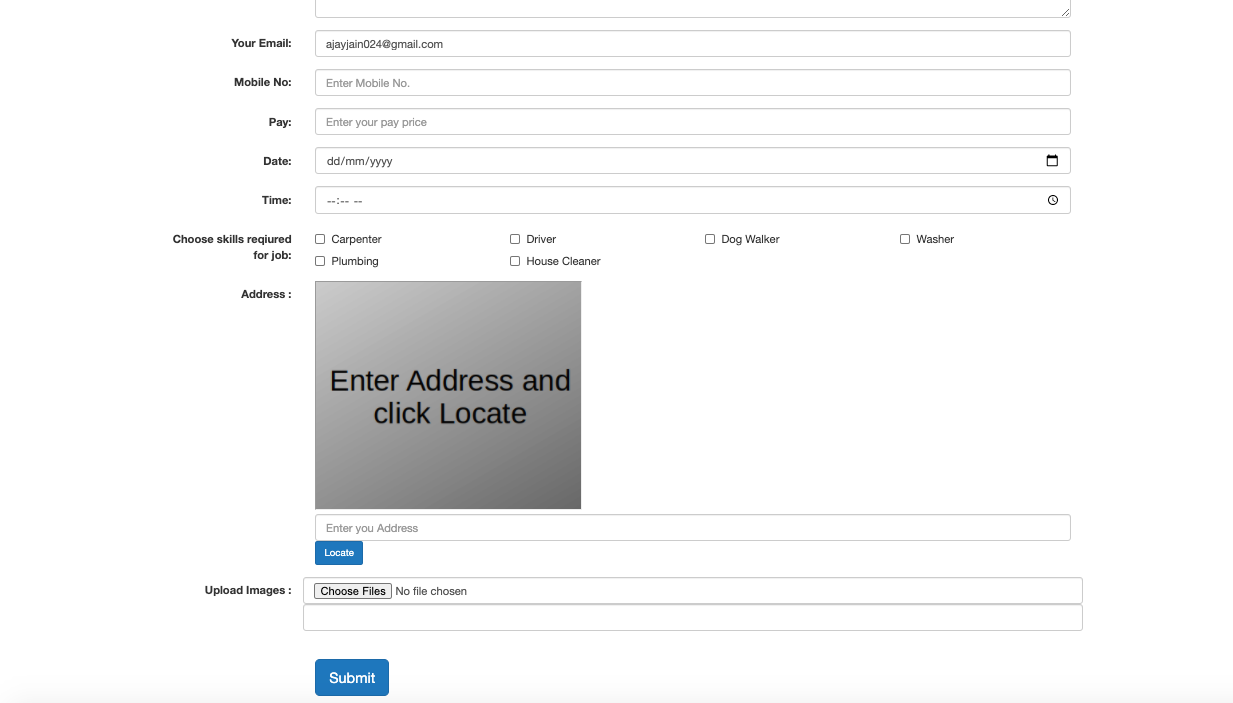
\includegraphics[width=15cm, height=8cm]{post job 1.png}


\subsection{Posted Job Responses}
This option in navigation is visible only if your profile type is both or job provider. Using this you will be able to see who have applied to the all the jobs you have posted with his details by clicking on view responses. There is another button mark as completed which helps you to mark job successfully completed.\\

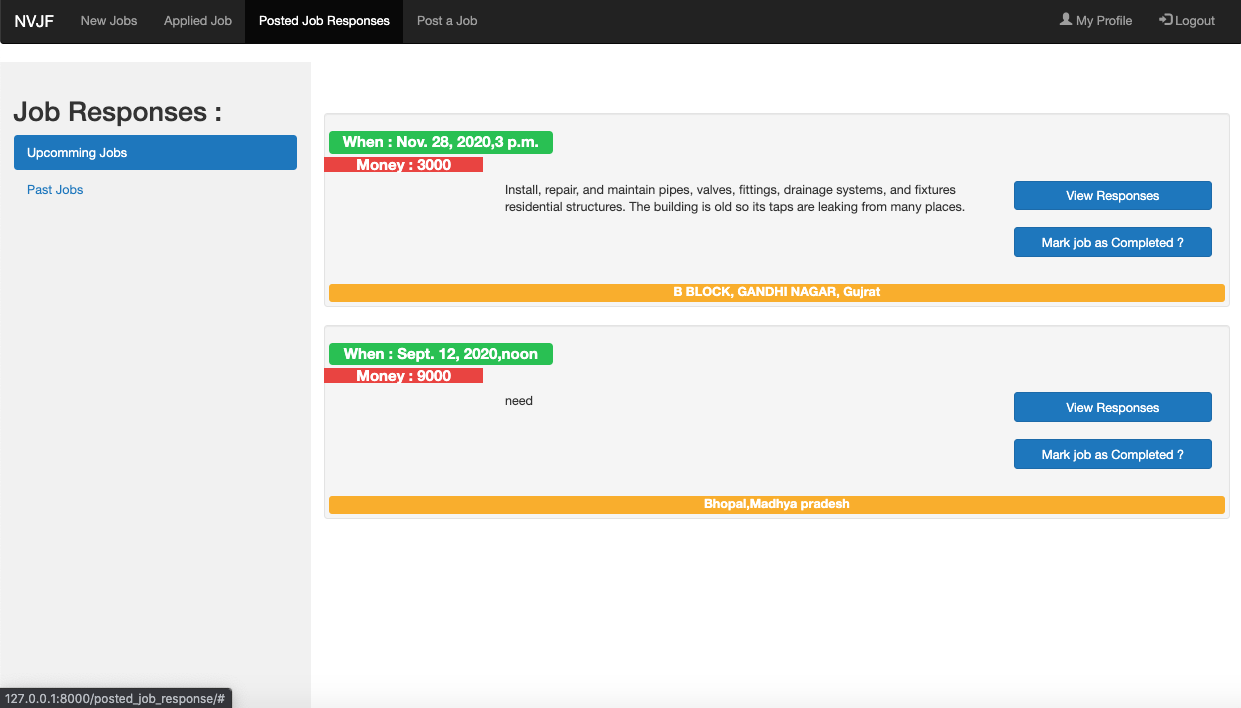
\includegraphics[width=15cm, height=8cm]{posted job upcoming.png}

\subsection{View Response}
If you click on view response button you will be able to see all the job seeker who have applied to the job you have posted and then you will be able to select a one or more person for the job depending on requirement by clicking on select button which is provided adjacent to each job response you have got.\\

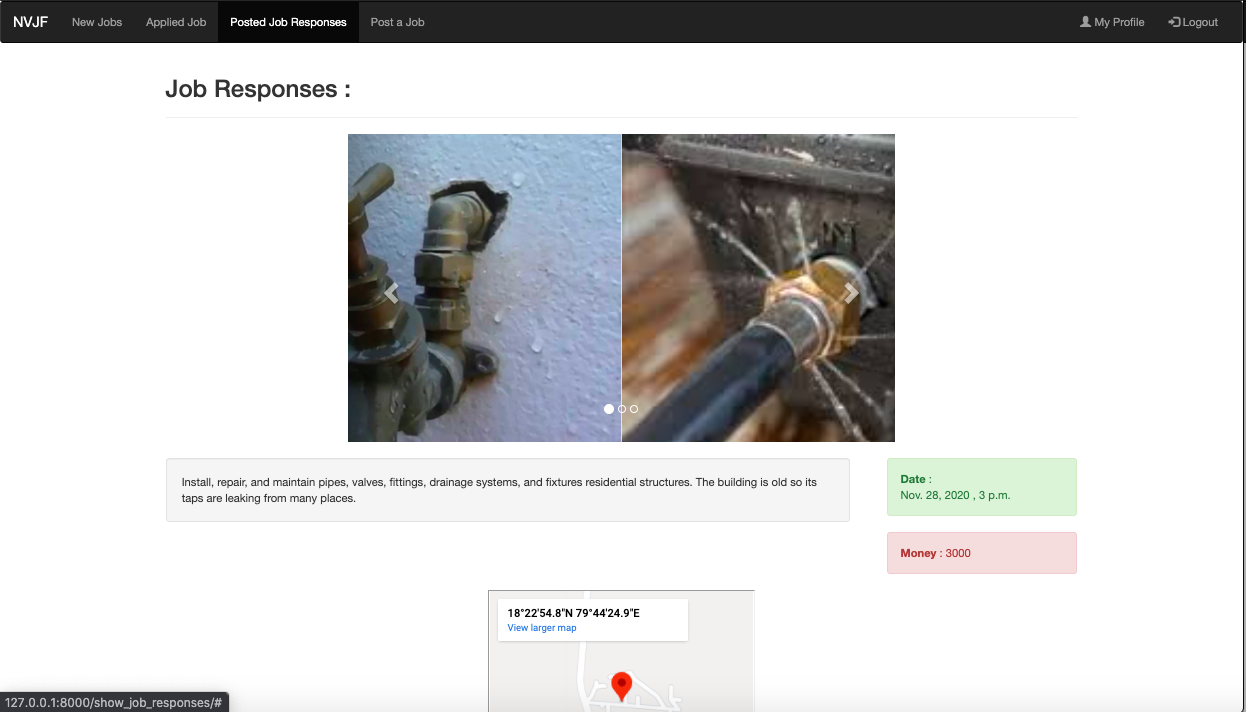
\includegraphics[width=15cm, height=8cm]{Job responses.png}
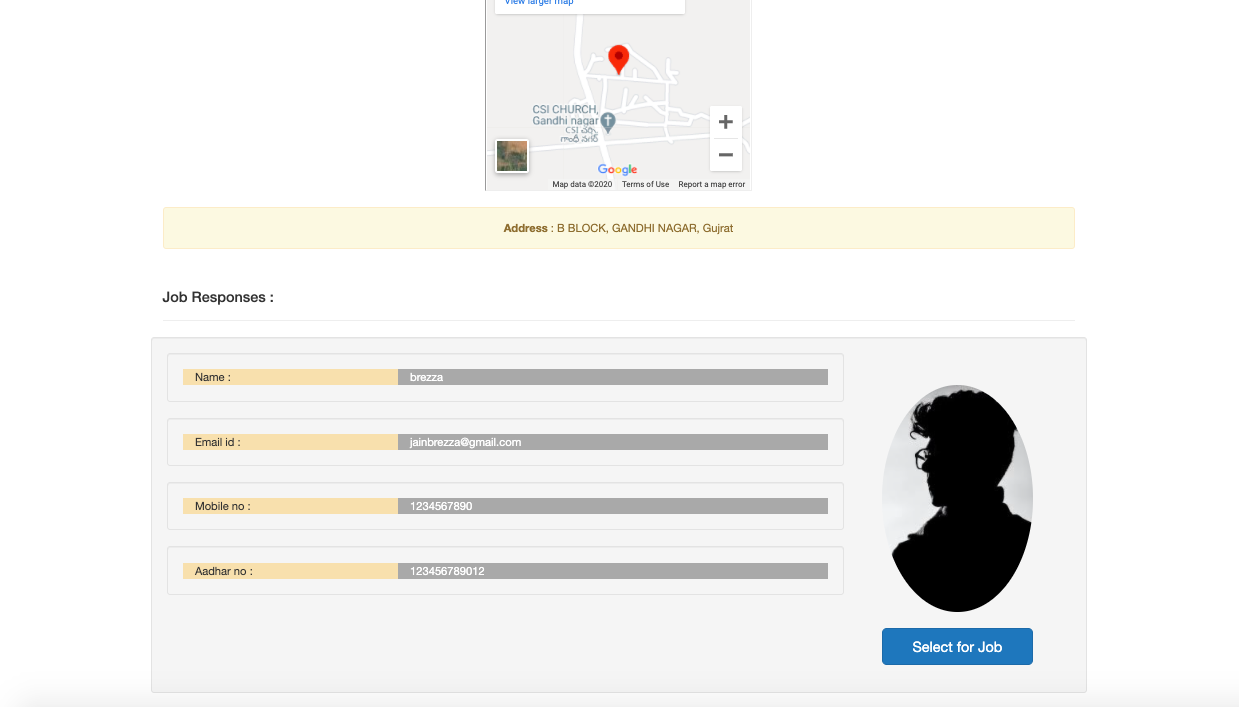
\includegraphics[width=15cm, height=8cm]{job responses 2.png}

\section{\textbf{System Design}}
\subsection{ER Diagram}

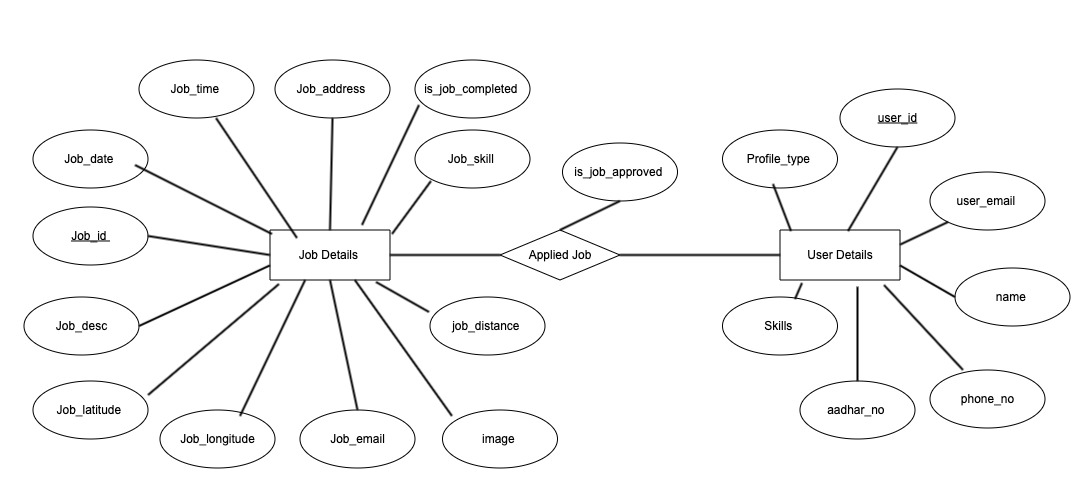
\includegraphics[width=15cm, height=8cm]{er_diagram.jpg}

\subsection{Use Case Diagram}

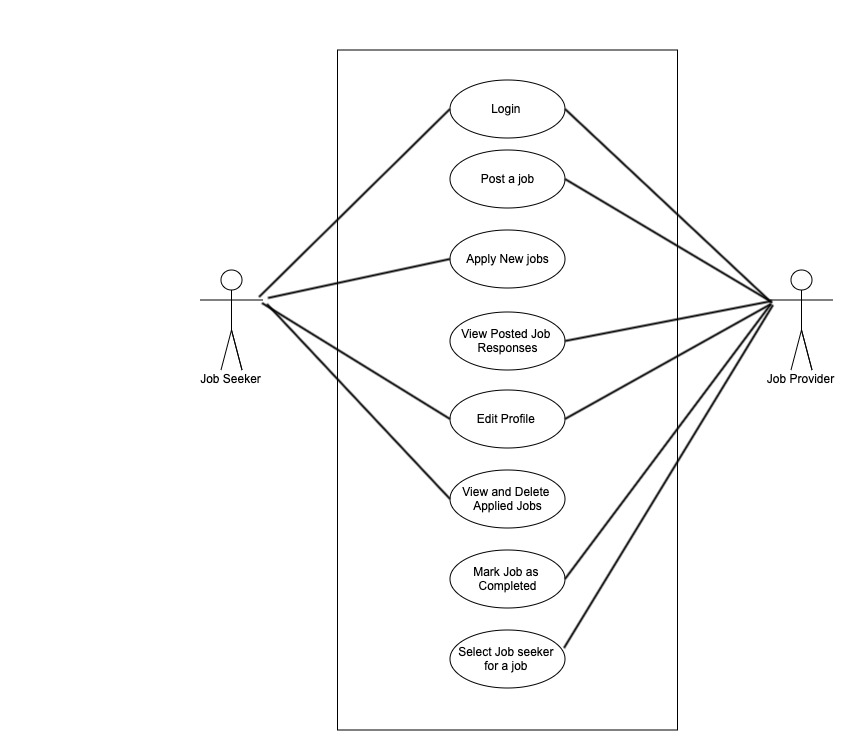
\includegraphics[width=15cm, height=8cm]{usecase.jpg}




\end{document}
